\chapter{MARCO TEORICO}

\section{Seguridad en la industria de la construcción}
\subsection{Importancia de la seguridad en el trabajo}
La industria de la construcción es uno de los sectores más riesgosos debido a la naturaleza de las actividades que se realizan en ella. Los accidentes laborales pueden tener consecuencias devastadoras, tanto para los trabajadores como para las empresas. Implementar medidas de seguridad adecuadas no solo previene lesiones, sino que también reduce los costos relacionados con la atención médica, la pérdida de productividad y las posibles sanciones legales. La seguridad en el trabajo es, por lo tanto, un pilar fundamental en la gestión de proyectos de construcción.

\subsection{Equipos de protección personal (EPP)}
Los EPP son dispositivos diseñados para proteger a los trabajadores de riesgos potenciales en su entorno de trabajo. Estos incluyen cascos de seguridad, guantes, gafas, arneses, y ropa de alta visibilidad, entre otros como se muestra en la figura \ref{fig:epp}. El uso adecuado de los EPP es fundamental para reducir la probabilidad de accidentes graves. Las regulaciones internacionales, como la ISO 45001, y locales, como la norma G-050 en Perú, establecen los estándares mínimos para la implementación y uso de estos equipos en las obras de construcción.

\begin{figure}[!ht]
  \centering
  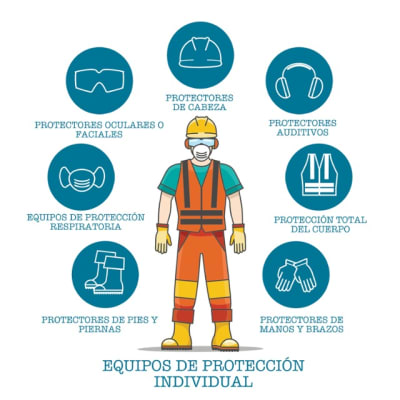
\includegraphics[width=.49\linewidth]{images/epp.jpg}
  \caption{Equipos de protección personal individual.}
  \label{fig:epp}
\end{figure}

\subsection{Uso del casco de seguridad}

El casco es uno de los elementos más importantes del EPP, diseñado como se muestra en la figura \ref{fig:casco} para proteger la cabeza del trabajador de impactos con objetos que caen o golpean. Según las normativas internacionales y locales, su uso es obligatorio en prácticamente todas las actividades dentro de una obra. Sin embargo, su efectividad depende del uso correcto y constante. La supervisión del cumplimiento de esta medida es uno de los principales retos en las obras, y es donde las tecnologías emergentes pueden marcar la diferencia.

\begin{figure}[!ht]
  \centering
  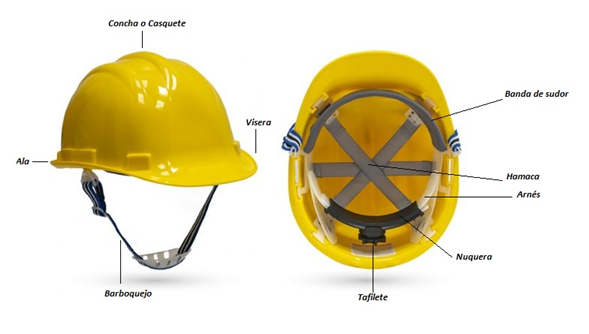
\includegraphics[width=.49\linewidth]{images/casco.png}
  \caption{Estructura de un casco de seguridad.}
  \label{fig:casco}
\end{figure}

\section{Inteligencia artificial y visión por computadora}

\subsection{Definición y conceptos básicos}

La inteligencia artificial (IA) es una rama de la informática que busca crear sistemas capaces de realizar tareas que normalmente requieren inteligencia humana, como el reconocimiento de patrones, la toma de decisiones y la predicción. La visión por computadora es un subcampo de la IA que se enfoca en permitir que las máquinas “vean” e interpreten el entorno a través de imágenes o videos, extrayendo información útil como la identificación de objetos, clasificación de imágenes o análisis de patrones.

\subsection{Detección de objetos}

La detección de objetos es una técnica dentro de la visión por computadora que se utiliza para localizar e identificar varios objetos dentro de una imagen o un video como se muestra en la figura \ref{fig:object_detection}. Esta técnica combina la clasificación de imágenes con la localización de objetos, indicando en qué área de la imagen se encuentra el objeto. Se han desarrollado múltiples modelos para esta tarea, siendo YOLO (You Only Look Once) uno de los más eficaces y populares debido a su velocidad y precisión.

\begin{figure}[!ht]
  \centering
  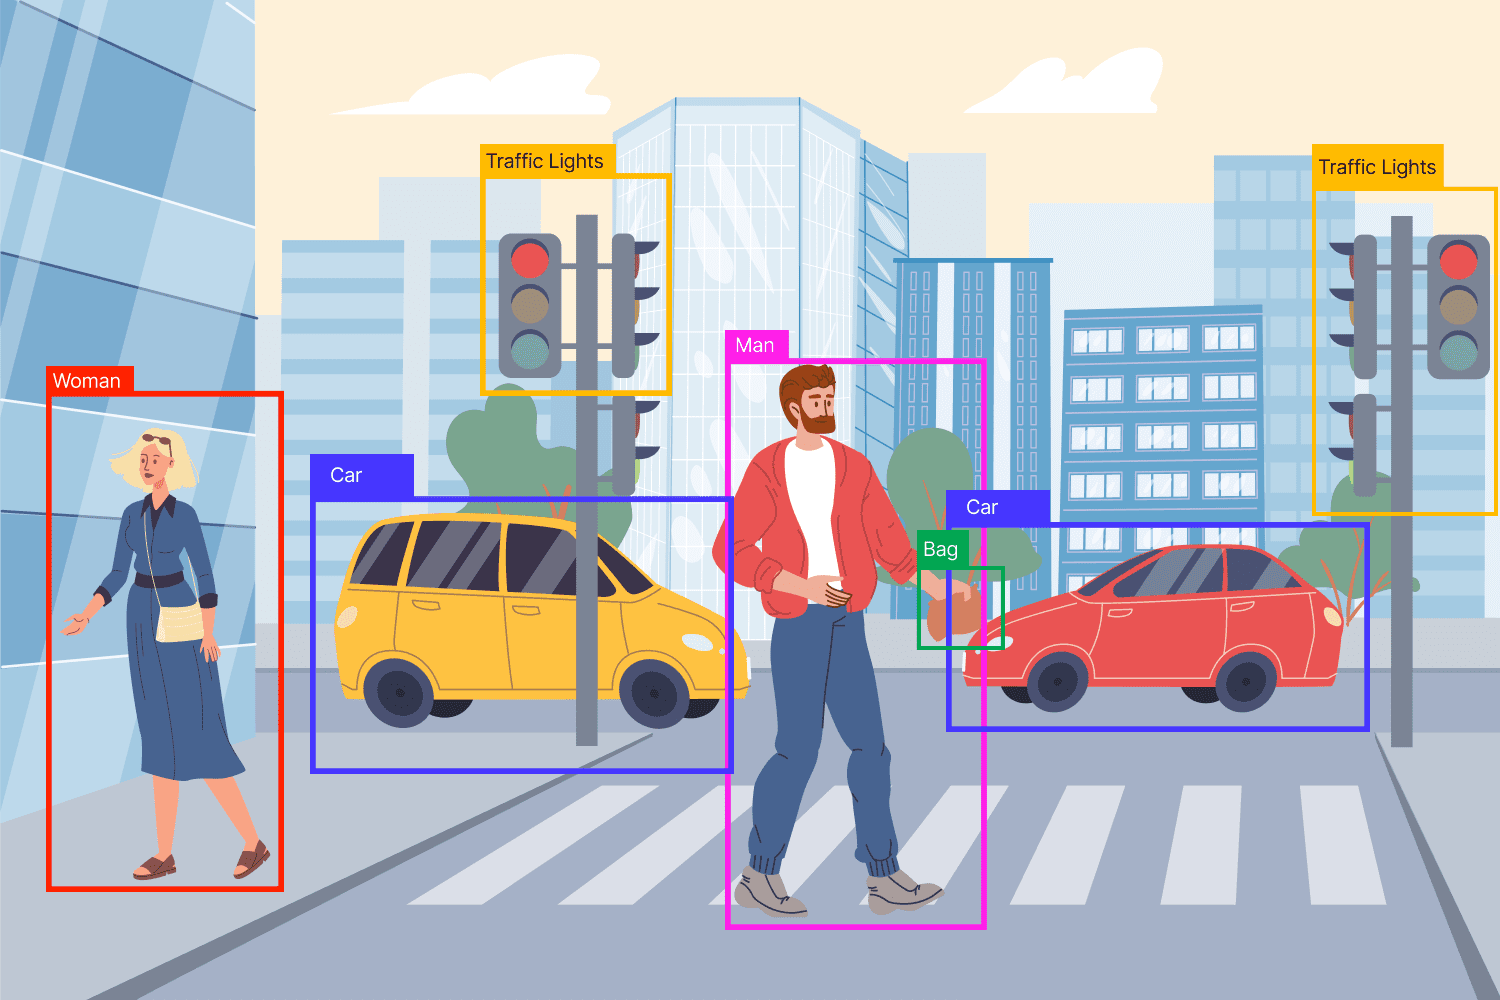
\includegraphics[width=.49\linewidth]{images/object_detection.png}
  \caption{Ejemplo de detección de objetos dentro de una imagen.}
  \label{fig:object_detection}
\end{figure}

\section{Modelos de detección de objectos: YOLO}

\subsection{Historia y evolución de YOLO}

YOLO es una familia de modelos de inteligencia artificial para la detección de objetos en imágenes, creado por Joseph Redmon en 2016. Su principal ventaja radica en su capacidad de detectar objetos en tiempo real con alta precisión, a diferencia de otros modelos que requieren múltiples pasos para lograr este objetivo. Desde su lanzamiento, ha pasado por varias versiones como se muestra en la figura \ref{fig:yolo_evolution}, mejorando en precisión, velocidad y capacidad de generalización en cada iteración. La versión más reciente, YOLOv8, incorpora las últimas innovaciones en redes neuronales profundas.

\begin{figure}[!ht]
  \centering
  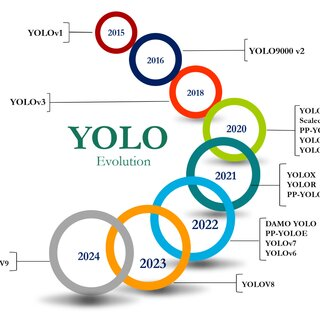
\includegraphics[width=.49\linewidth]{images/yolo_evolution.jpg}
  \caption{Evolución de las versiones de YOLO.}
  \label{fig:yolo_evolution}
\end{figure}

\subsection{Características de YOLOv8}

YOLOv8 es la última versión estable de la serie YOLO, y se distingue por su arquitectura optimizada \ref{fig:yolo_architecture}, lo que permite detectar objetos con mayor rapidez y exactitud. Sus principales características incluyen la capacidad de operar en tiempo real, ser más ligero en comparación con sus predecesores, y lograr un balance óptimo entre precisión y velocidad. YOLOv8 ha sido diseñado para integrarse fácilmente en aplicaciones de seguridad, donde la detección precisa y rápida es crucial.

\begin{figure}[!ht]
  \centering
  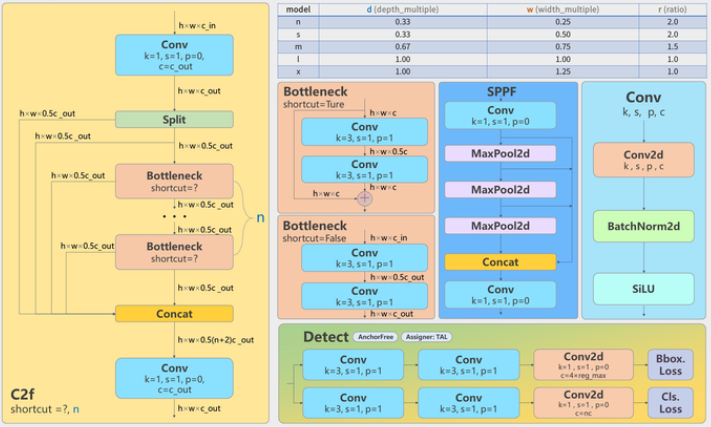
\includegraphics[width=.49\linewidth]{images/yolo_architecture.png}
  \caption{Arquitectura de modelo YOLOv8.}
  \label{fig:yolo_architecture}
\end{figure}

\subsection{Aplicaciones de YOLO en la seguridad}

El uso de YOLO en el ámbito de la seguridad ha demostrado ser altamente efectivo, especialmente en la detección de equipos de protección personal (EPP) como se muestra en la figura \ref{fig:yolo_application}. En entornos como las obras de construcción, la capacidad de este modelo para detectar la presencia o ausencia de cascos de seguridad en tiempo real representa una herramienta valiosa para mejorar la supervisión y cumplimiento de las normativas de seguridad.

\begin{figure}[!ht]
  \centering
  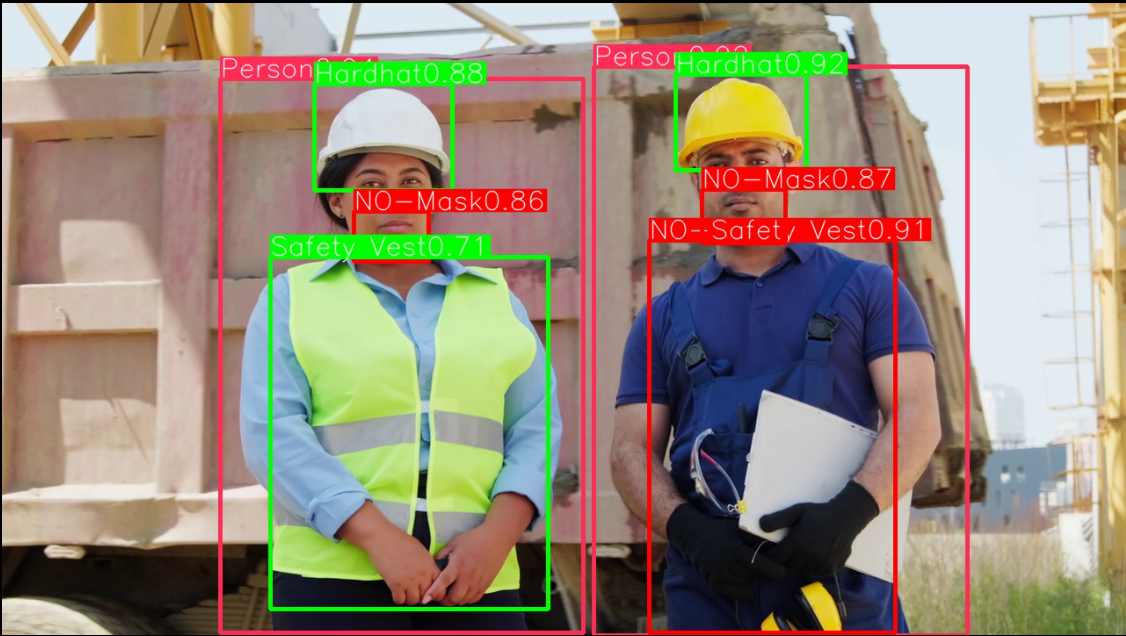
\includegraphics[width=.49\linewidth]{images/yolo_application.png}
  \caption{Aplicación de YOLOv8 en la detección de equipos de protección personal (EPP).}
  \label{fig:yolo_application}
\end{figure}

\section{Técnicas de preprocesamiento de imágenes}

\subsection{Redimensionamiento y recorte de imágenes}

El redimensionamiento y recorte de imágenes mostrado en la figura \ref{fig:image_cropping} son etapas fundamentales en el preprocesamiento de datos para la detección de objetos. En el caso de YOLOv8, es necesario ajustar las imágenes a un tamaño estándar (640x640 píxeles) para que el modelo pueda procesarlas eficientemente. Se pueden utilizar varias técnicas de recorte, como recorte desde la izquierda, corte centrado, y corte con superposición, para garantizar que todas las áreas importantes de la imagen sean utilizadas.

\begin{figure}[!ht]
  \centering
  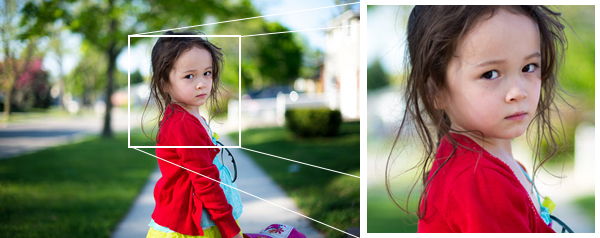
\includegraphics[width=.49\linewidth]{images/cropping.jpg}
  \caption{Recorte de imagen en una region especifica.}
  \label{fig:image_cropping}
\end{figure}

\subsection{Aumentación de datos}

La aumentación de datos es una técnica que se utiliza para expandir el conjunto de datos mediante la creación de variaciones \ref{fig:data_augmentation} de las imágenes originales. Estas variaciones pueden incluir rotaciones, volteos, y cambios en la iluminación. Este proceso ayuda a aumentar la diversidad del dataset, lo que mejora la capacidad del modelo para generalizar y manejar distintos tipos de imágenes.

\begin{figure}[!ht]
  \centering
  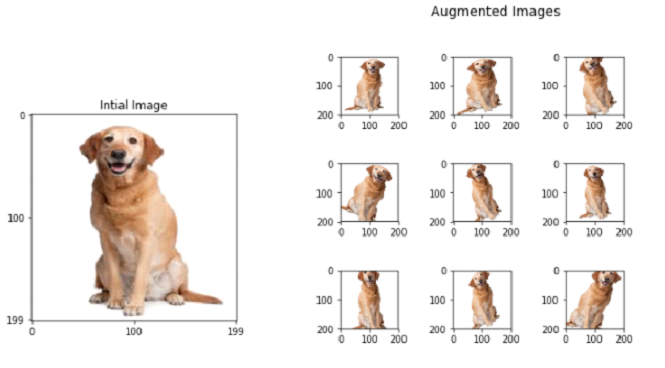
\includegraphics[width=.49\linewidth]{images/data_augmentation.png}
  \caption{Aumentación de images con diferentes configuraciones.}
  \label{fig:data_augmentation}
\end{figure}

\section{Herramientas y plataformas de etiquetado}

\subsection{Introducción al etiquetado de imágenes}

El etiquetado de imágenes es el proceso mediante el cual se asignan etiquetas o clases a objetos dentro de una imagen. En el caso de los EPPs, se etiqueta la presencia de cascos, lo que permite que el modelo aprenda a reconocer estos elementos. El etiquetado es un paso crucial, ya que los datos mal etiquetados pueden afectar negativamente el rendimiento del modelo.

\subsection{Roboflow: Plataforma de etiquetado}

Roboflow es una plataforma  \ref{fig:roboflow_labeling} popular para la gestión y etiquetado de imágenes en proyectos de visión por computadora. Ofrece una interfaz intuitiva para cargar, etiquetar y preparar datasets para ser utilizados en modelos como YOLOv8. La plataforma también facilita la exportación de los datos en formatos compatibles con YOLO, optimizando el flujo de trabajo para la creación de modelos personalizados.

\begin{figure}[!ht]
  \centering
  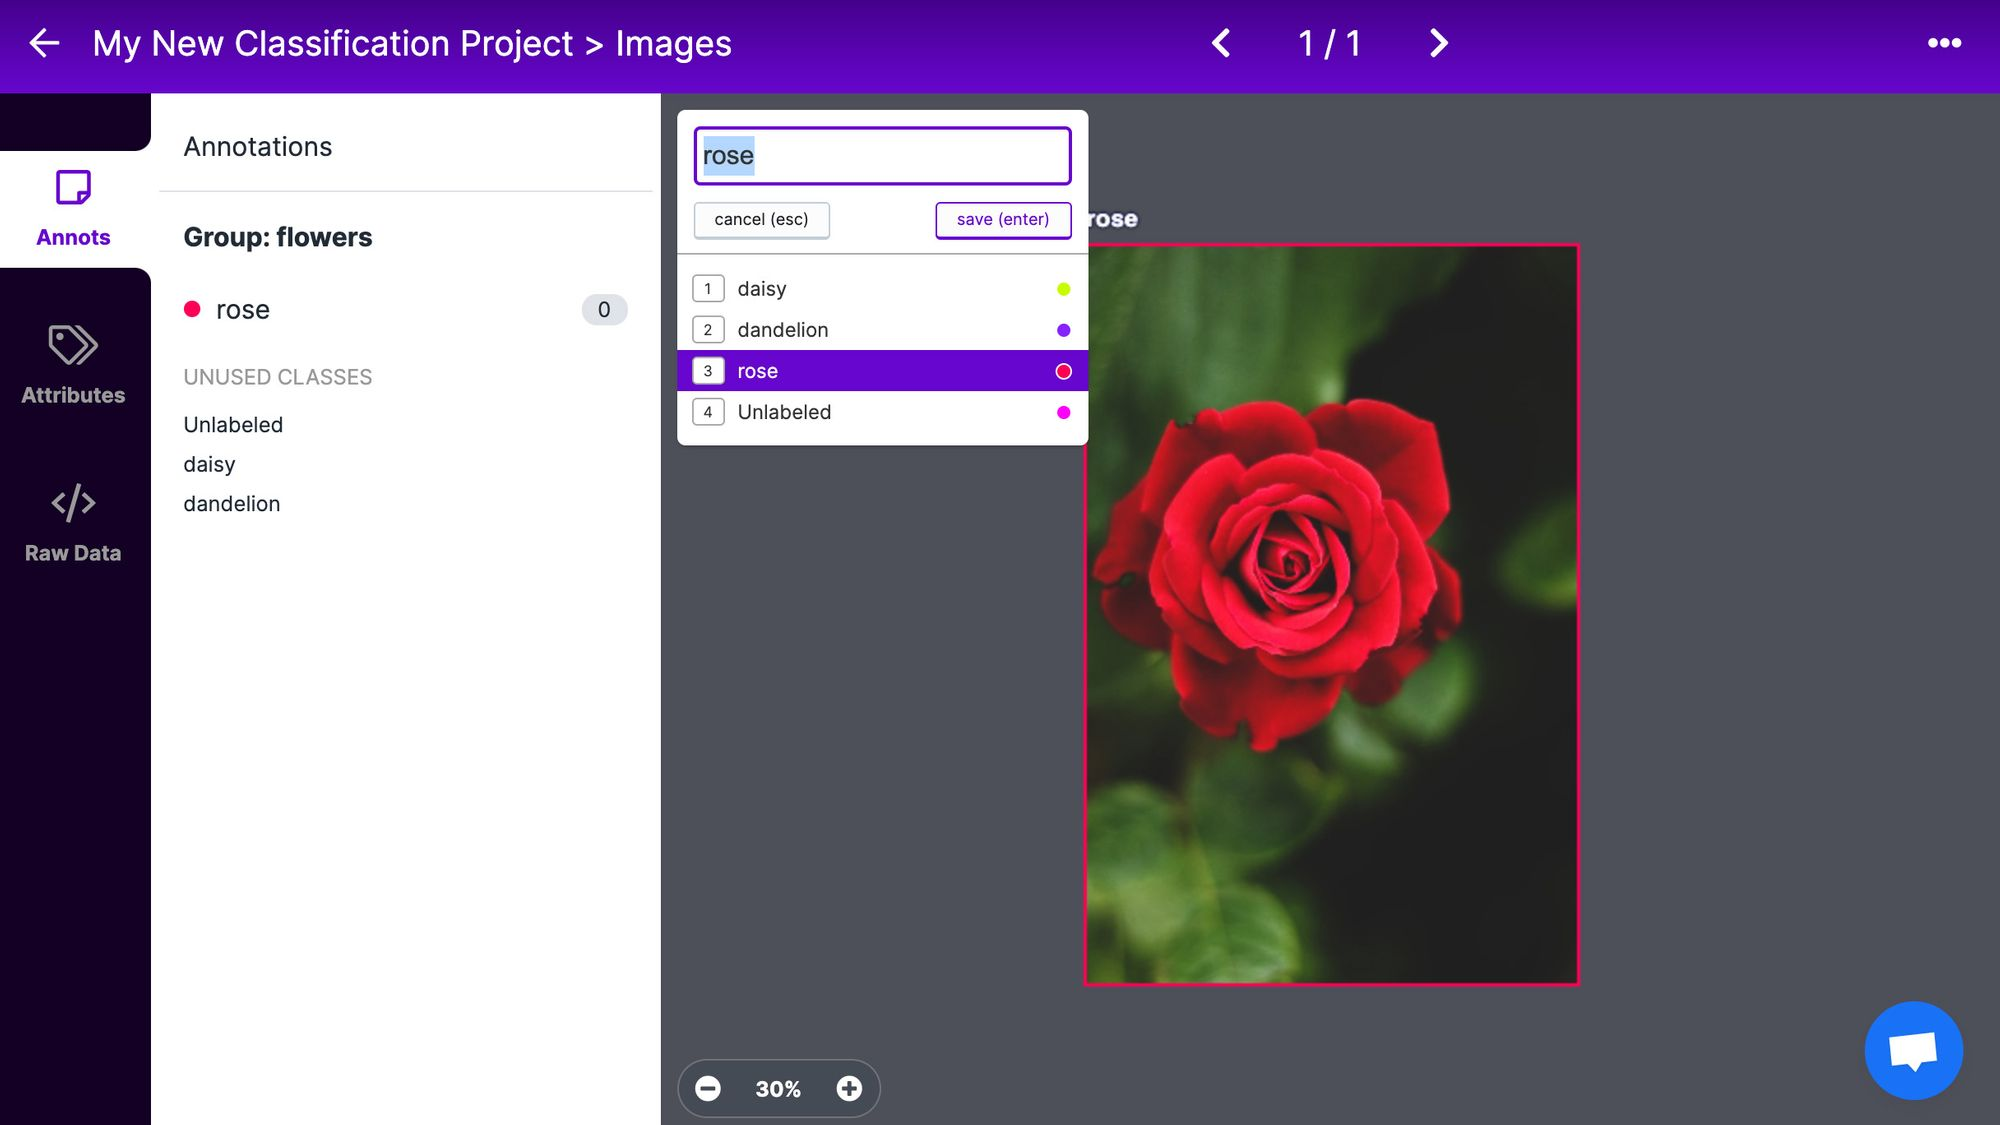
\includegraphics[width=.49\linewidth]{images/roboflow_labeling.jpg}
  \caption{Interfaz de Roboflow para el etiquetado de clases.}
  \label{fig:roboflow_labeling}
\end{figure}



